\chapter{Estrutura de Dados Hierárquica }

As árvores são estruturas de dados que são bastante apropriadas para representar dados dispostos de maneira hierárquica. Por exemplo, podemos representar a hierarquia do sistema de arquivos no sistema operacional linux usando uma árvore.


\begin{figure}[htbp]
\centering
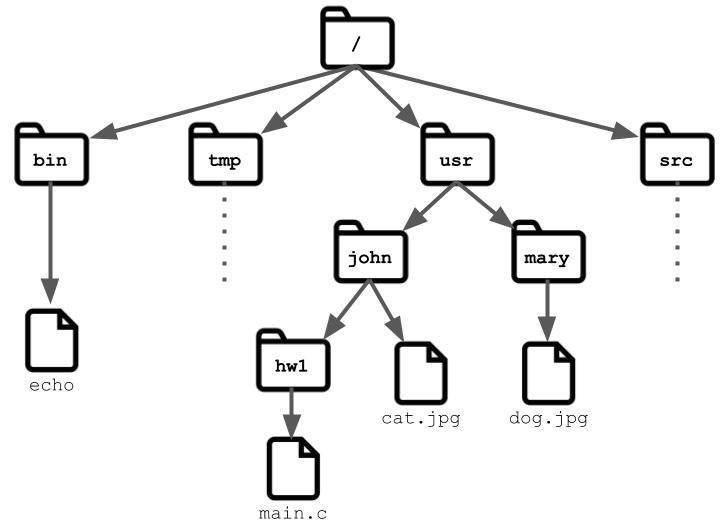
\includegraphics[width=.6\textwidth]{images/file_system.png}
\label{fig:exampleFig2}
\end{figure}

Expressões matemáticas com operadores binários podem ser representados utilizando árvores de expressões. Na figura \ref{fig::tree_expression}, mostra a árvore de expressão da (a+b)*c+7.

\begin{figure}[htbp]
\centering
\label{fig::tree_expression}
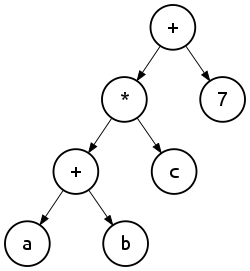
\includegraphics[scale=0.5]{images/250px-Exp-tree-ex-11.svg.png}
\label{fig:exampleFig2}
\caption{Árvore de expressão da expressão (a+b)*c+7}
\end{figure}

A representação de uma expressão no formato de árvore tem algumas vantagens importantes:

\begin{itemize}
    \item A árvore de expressão não precisa guardar delimitadores e símbolos de pontuação.
    \item A representação hierárquica deixa claro a ordem de avaliação dos operadores.
    \item Você pode guardar informações extra sobre os operandos e operadores na árvore de expressão.
\end{itemize}



\section{Árvore de Expressão}

Uma expressão aritmética é uma sequência de texto que possui estrutura de recursiva de formação. Uma expressão aritmética pode ser construída a partir de números, variáveis, operadores binários como +,-,* e / e alguns símbolos de pontução como '(' e ')'. 

Uma expressão aritmética (EXP) pode ser definida da seguinte maneira:

\begin{itemize}
\item Seja $\alpha$ uma sequência de texto representando um número então $\alpha \in EXP$.
\item Seja $\alpha$ uma sequência de texto representando uma variável então $\alpha \in EXP$.
\item Seja $\alpha, \beta \in EXP$  então $\alpha + \beta \in EXP, \alpha - \beta \in EXP, \alpha * \beta \in EXP$ e $\alpha / \beta \in EXP$.
\end{itemize} 


Para construir uma estrutura de dados para representar uma expressão dada, precisamos construir uma árvore onde cada nó da árvore pode ser qualquer uma das diferentes formas que essa expressão pode assumir. Por exemplo, em um árvore de expressão aritmética, um nó pode representar uma constante, uma variável ou uma operação binária como a soma, subtração, multiplicação ou divisão. Observe que cada esses tipos de nós tem uma quantidade de filhos diferentes.

Uma maneira de definir essa estrutura de dados é construir uma única classe para os nós com todas as informações para os diferentes tipos de nós como um rótulo para indicar cada tipo de nó da seguinte maneira:

\begin{minted}
[
frame=lines,
bgcolor=LightGray,
fontsize=\footnotesize,
linenos
]
{C++}
class exp {
    public:
    typedef enum { NUM, VAR, BINOP} exp_type;
    exp_type type;
    int value;
    string name;
    char op;
    exp * left;
    exp * right;
    exp(int value);
    exp(string name);
    exp(char op, exp * left, exp * right);
};
\end{minted}

A função para imprimir uma árvore de expressão seria da seguinte maneira:


\begin{minted}
[
frame=lines,
bgcolor=LightGray,
fontsize=\footnotesize,
linenos
]
{C++}
void print(exp * e){
    switch(e->type){
        case exp::NUM:
            cout << e->value;
            break;
        case exp::VAR:
            cout << e->name;
            break;
        case exp::BINOP:
            print(e->left);
            cout << e->op;
            print(e->right);
            break;
    }

}
\end{minted}

Essa implementação possui algumas desvantagens:

\begin{itemize}
\item Como temos apenas uma classe para representar os diferentes tipos de nós, qualquer alteração ou extensão precisar alterar essa classe.
\item A quantidade de filhos não interfere na quantidade de memória utilizada para cada nó.
\item Ao usar um nó, precisamos sempre checar seu rótulo para realizar as operações de maneira adequada.
\end{itemize}

Uma outra maneira de implementar uma árvore de expressão é utilizando uma hierarquia de herança dos diferentes tipos de nós de uma árvore de expressão. Vamos definir uma classe base e em seguida adicionar as subclasses, uma para cada tipo de nó.

Classe Base:

\begin{minted}
[
frame=lines,
bgcolor=LightGray,
fontsize=\footnotesize,
linenos
]
{C++}
class exp {
    public:
    virtual void print() = 0; // Pure virtual
};
\end{minted}

Hierarquia de Herança:

\begin{minted}
[
frame=lines,
bgcolor=LightGray,
fontsize=\footnotesize,
linenos
]
{C++}
class exp_num : public exp {
    int value;
    public:
    exp_num(int value);
    virtual void print() {
        cout << value;
    }
};

class exp_var : public exp {
    
    string name;
    public:
    exp_var(string name);
    virtual void print() {
        cout << name;
    }
};


struct exp_op : public exp {
    char op;
    exp* left;
    exp* right;
    public:
    exp_op(char op, exp * left, exp * right);
    virtual void print() {
        left->print();
        cout << op;
        right->print();
    }
};

\end{minted}

Uma árvore de expressão pode ser construída da seguinte maneira:
\begin{minted}
[
frame=lines,
bgcolor=LightGray,
fontsize=\footnotesize,
linenos
]
{C++}
    exp * e =   new exp_op('+', 
                new exp_num(2),
                new exp_num(3)
                );
    e->print();

\end{minted}

\section{Construindo uma árvore de expressão}

Considere uma expressão na notação polonesa reversa (notação pós-fixa). A construção da árvore de expressão pode ser realizada com as seguintes regras:

\begin{enumerate}
    \item Se o símbolo é operando então crie um ponteiro para nó da árvore para o operando e empilhe um ponteiro para um nó representado pelo operando.
    \item Se o símbolo é um operador binário, desempilhe dois ponteiros para nós e empilhe na pilha um ponteiro para um nó representando o operador binário com dois filhos.
\end{enumerate}

Considere o processo de criação da árvore de expressão para a seguinte expressão: a b + c d e + * * 


\begin{enumerate}

\item Dois ponteiros para nós são criados para os dois primeiros operandos e empilhados na pilha.

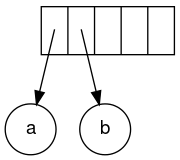
\includegraphics[scale=0.5]{images/passo1.png}

\item Um operador é encontrado, dois ponteiros são retirados da pilha e um novo nó é empilhado.

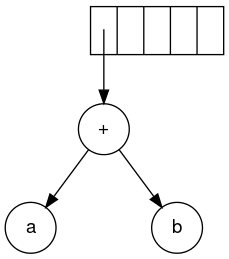
\includegraphics[scale=0.5]{images/passo2.png}

\item Três ponteiros para nós são criados para os próximos três operandos e eles são empilhados na pilha.

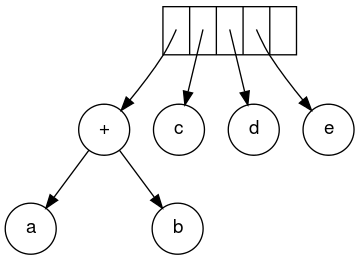
\includegraphics[scale=0.5]{images/passo3.png}

\item Um operador é encontrado, dois ponteiros são retirados da pilha e um novo ponteiro nó é empilhado.

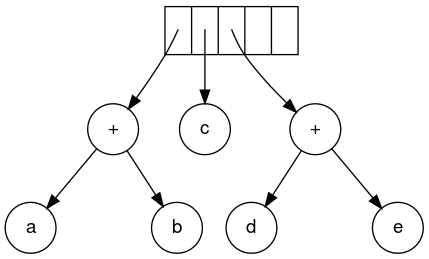
\includegraphics[scale=0.5]{images/passo4.png}

\item Um operador é encontrado, dois ponteiros são retirados da pilha e um novo ponteiro nó é empilhado.

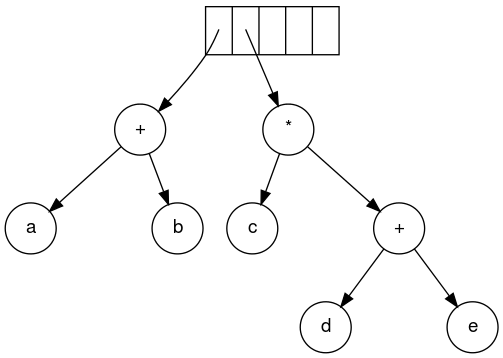
\includegraphics[scale=0.5]{images/passo5.png}

\item Um operador é encontrado, dois ponteiros são retirados da pilha e um novo ponteiro para nó é empilhado.

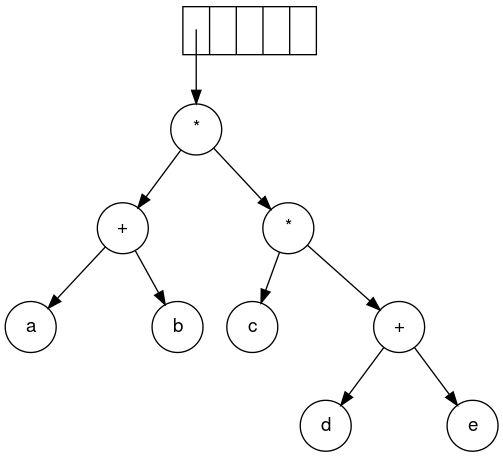
\includegraphics[scale=0.5]{images/passo6.png}


\end{enumerate}



\begin{minted}
[
frame=lines,
bgcolor=LightGray,
fontsize=\footnotesize,
linenos
]
{C++}
exp * read_postfix(vector <string> tokens){
    stack <exp *> st;

    for(string t : tokens){
        if( is_numeric(t) ){
            st.push( new exp_num(stoi(t)) );
        }
        else if( is_variable(t) ){
            st.push( new exp_var(t) );
        }else if( is_op(t) ){
            exp * r = st.top(); st.pop();
            exp * l = st.top(); st.pop();
            st.push( new exp_op(t.front(), l, r) );
        } 
    }
    return st.top();
}
\end{minted}



\section{Expressão Lógica}

Uma expressão lógica é uma sequência de texto que utiliza constantes (true, false), variáveis proposicionais e operadores lógicos como ($\neg, \wedge, \vee, \to, \leftrightarrow$).

O conjunto da expressões lógicas (EXPLOG) bem-formadas pode ser definido da seguinte maneira:

\begin{itemize}
    \item Se $\alpha$ é uma constante, então $ \alpha\in  EXPLOG$.
    \item Se $\alpha$ é uma variável proposicional, então $ \alpha\in  EXPLOG$.
    \item Se $\alpha \in EXPLOG$ então 
    $$\neg \alpha \in EXPLOG$$.
    \item Se $\alpha,\beta \in EXPLOG$ então 
    $$\alpha \vee \beta, \alpha \wedge \beta, \alpha \to \beta, \alpha \leftrightarrow \beta$$.
\end{itemize}

Novamente, vamos recorrer uma hierarquia de herança para representar uma expressão lógica da seguinte maneira:


\begin{minted}
[
frame=lines,
bgcolor=LightGray,
fontsize=\footnotesize,
linenos
]
{C++}
class logical {
  public:
    virtual void print() = 0;
    
};

class log_const : public logical {
  public:
    log_const(bool value) : value(value) {}
    void print() { 
        cout << value ? "true" : "false";
    }
  private:
    bool value;
};

class log_prop : public logical {
  public:
    log_prop(string name) : name(name) {}
    
    void print() {
        cout << name;
    }
  private:
    string name;
};

class log_neg : public logical {
  public:
    log_neg(logical * inner) : inner(inner) {}
    void print() {
        cout << "~";
        inner->print();
    }
    
  private:
    logical* inner;
};

class log_op : public logical {
  public:
    log_op(string op, logical * l, logical * r) : op(op), left(l), right(r) {}
    void print() {
        cout << "("; left->print(); cout << op; right->print(); cout << ")";
    }
  private:
    string op;
    logical * left;
    logical * right;
};

\end{minted}

O processo de construção de uma árvore de expressão lógica a partir de uma expressão na notação pós-fixa segue o mesma ideia:


\begin{minted}
[
frame=lines,
bgcolor=LightGray,
fontsize=\footnotesize,
linenos
]
{C++}
logical * read_postfix(vector <string> tokens){
    stack <logical *> st;

    for(string t : tokens){
        
        if( is_bool(t) ){
            
            st.push( new log_const( t == "true" ) );
        }
        else if( is_variable(t) ){
            
            st.push( new log_prop(t) );
        }else if( t == "~"){
            logical * inner = st.top(); st.pop();
            st.push( new log_neg(inner) );
        }
        else if( is_op(t) ){
            logical * r = st.top(); st.pop();
            logical * l = st.top(); st.pop();

           
            st.push( new log_op(t , l, r) );
        } 
    }
    return st.top();
}
\end{minted}

Imagine que você queira encontrar uma expressão lógica equivalente sem a utilização do operador $\to$. Você pode utilizar a seguinte regra de equivalência:

$$
\alpha \to \beta \equiv \neg \alpha \vee \beta
$$

O processo de remoção do implicação pode ser definido de maneira recursiva. Seja REMOVE\_IMPLIES($\alpha$) uma função que devolve uma expressão lógica equivalente a $\alpha$ sem o operador $\to$.

\begin{itemize}
    \item Se $\alpha$ é uma constante, então $REMOVE\_IMPLIES(\alpha) = \alpha$.
    \item Se $\alpha$ é uma variável proposicional, então $REMOVE\_IMPLIES(\alpha) = \alpha$.
    \item Se $\neg \alpha \in EXPLOG$ então 
    $$REMOVE\_IMPLIES(\neg \alpha) = \neg REMOVE\_IMPLIES(\alpha)$$
    \item Se $\alpha \vee \beta \in EXPLOG$ então 
    $$REMOVE\_IMPLIES(\alpha \vee \beta) = REMOVE\_IMPLIES(\alpha) \vee REMOVE\_IMPLIES(\beta)$$.
    \item Se $\alpha \wedge \beta \in EXPLOG$ então 
    $$REMOVE\_IMPLIES(\alpha \wedge \beta) = REMOVE\_IMPLIES(\alpha) \wedge REMOVE\_IMPLIES(\beta)$$.
    \item Se $\alpha \leftrightarrow \beta \in EXPLOG$ então 
    $$REMOVE\_IMPLIES(\alpha \leftrightarrow \beta) = REMOVE\_IMPLIES(\alpha) \leftrightarrow REMOVE\_IMPLIES(\beta)$$.
    \item Se $\alpha \to \beta \in EXPLOG$ então 
    $$REMOVE\_IMPLIES(\alpha \to \beta) = \neg REMOVE\_IMPLIES(\alpha) \vee REMOVE\_IMPLIES(\beta)$$.
\end{itemize}

Essa função pode ser implementada sem utilizar a hierarquia de herança da seguinte maneira:

\begin{minted}
[
frame=lines,
bgcolor=LightGray,
fontsize=\footnotesize,
linenos
]
{C++}
logical * remove_implies(logical * exp){

  log_neg * exp_neg = dynamic_cast<log_neg*>(exp);

  if( exp_neg != nullptr){
    
    return new log_neg( remove_implies( exp_neg->inner) );
  }
  else{
    log_op * exp_op = dynamic_cast<log_op*>(exp);

    if( exp_op == nullptr)
    {
      return exp;
    }
    else
    {
      logical * l = remove_implies( exp_op->left );
      logical * r = remove_implies( exp_op->right);
        
      if( exp_op->op == "->")
      {  
        return new log_op("\\/", new log_neg(l), r);
      }
      else
        return new log_op(exp_op->op, l, r);
    }
  }

}

\end{minted}


\section{Árvore Binária}

Uma árvore binária é uma estrutura de dados genéricas para representar uma relação hierárquica em que cada nó tem no máximo 2 filhos. Na nossa modelagem, uma árvore binária será representada por um classe TreeNode com um valor que chamaremos key e dois ponteiros para TreeNode chamado left, right. 


\begin{minted}
[
frame=lines,
bgcolor=LightGray,
fontsize=\footnotesize,
linenos
]
{C++}
template <typename T> 
class NodeTree{
    public:
    T key;
    NodeTree<T> * left;
    NodeTree<T> * right;
    NodeTree(T key) : key(key), left(nullptr), right(nullptr) {};
    NodeTree(T key, NodeTree * l, NodeTree * r) : key(key), left(l), right(r) {};    
};
\end{minted}


A primeira função que criaremos será a função \texttt{createTree}. Essa função vai receber um vector keys com as chaves que serão armazenadas na árvore e um outro vector parent guardando o índice do nó pai para nó da árvore. Inicialmente, criaremos um vetor de nós da árvore. Para cada valor no vector keys, criaremos uma nó de uma árvore. Note que os dois ponteiros dos filhos da esquerda (left) e direita (right) vão ser inicializados com nullptr. A medida que fomos processando o vector parent, colocaremos o primeiro nó filho na esquerda e o segundo ó filho na direita.


\begin{minted}
[
frame=lines,
bgcolor=LightGray,
fontsize=\footnotesize,
linenos
]
{C++}
template <typename T> 
NodeTree<T> * createTree( vector<T> keys, vector<int> parent){

    NodeTree<T>* tree[keys.size()];
    NodeTree<T>* root;
    for(int i = 0; i < keys.size(); i++){
        tree[i] = new NodeTree<T>(keys[i]);
    }
    for(int i = 0; i < keys.size(); i++){
        if( parent[i] == -1)
            root = tree[i];
        else
        {
            NodeTree<T>* ptr = tree[ parent[i] ];
            if( ptr->left ){
                ptr->right = tree[i];
            }else{
                ptr->left = tree[i];
            }
        }
    }
    return root;
} 

\end{minted}

Em seguida, construíremos uma função \tetxtt{dotfile} para escrever um arquivo no formato dot para facilitar a visualização da nossa árvore binária:

\begin{minted}
[
frame=lines,
bgcolor=LightGray,
fontsize=\footnotesize,
linenos
]
{C++}

template <typename T>
void dotfileaux(ofstream & ofs, NodeTree<T> * ptr);


template <typename T>
void dotfile(NodeTree<T> * ptr)
{
    ofstream ofs ("bt.dot", ofstream::out);

    ofs << "digraph G {" << endl;

    dotfileaux(ofs, ptr);

    ofs << "}" << endl;

    ofs.close();

}

template <typename T>
void dotfileaux(ofstream & ofs, NodeTree<T> * ptr){
    static int nullcount = 0;
    if(ptr != nullptr){
        if(ptr->left){
            ofs << ptr->key << "->" << ptr->left->key  << ";" << endl;
            dotfileaux(ofs, ptr->left);
        }else{
            ofs << "null" << nullcount << " [shape=point];" << endl;
            ofs << ptr->key << "->" << "null" << nullcount << ";" << endl; 
            nullcount++;
        }
        if(ptr->right != nullptr){
            ofs << ptr->key << "->" << ptr->right->key  << ";" << endl;
            dotfileaux(ofs, ptr->right);
        }else{
            ofs << "null" << nullcount << " [shape=point];" << endl;
            ofs << ptr->key << "->" << "null" << nullcount << ";" << endl; 
            nullcount++;
        }
    }
} 

\end{minted}

Considerando a seguinte programa principal:


\begin{minted}
[
frame=lines,
bgcolor=LightGray,
fontsize=\footnotesize,
linenos
]
{C++}

int main(){
    vector<int> keys( {0,1,2,3,4,5,6,7});
    vector<int> parent({-1,0,0,1,2,2,4,4});
    auto root = createTree(keys, parent);
    dotfile(root);
}
\end{minted}

O programa principal acima escreve o seguinte arquivo dot:


\begin{minted}
[
frame=lines,
bgcolor=LightGray,
fontsize=\footnotesize,
linenos
]
{C++}

digraph G {
0->1;
1->3;
null0 [shape=point];
3->null0;
null1 [shape=point];
3->null1;
null2 [shape=point];
1->null2;
0->2;
2->4;
4->6;
null3 [shape=point];
6->null3;
null4 [shape=point];
6->null4;
4->7;
null5 [shape=point];
7->null5;
null6 [shape=point];
7->null6;
2->5;
null7 [shape=point];
5->null7;
null8 [shape=point];
5->null8;
}
\end{minted}

Você pode utilizar algum visualizador online de arquivos no formato dot \footnote{ \url{ https://dreampuf.github.io/GraphvizOnline/}} obtendo a seguinte imagem:

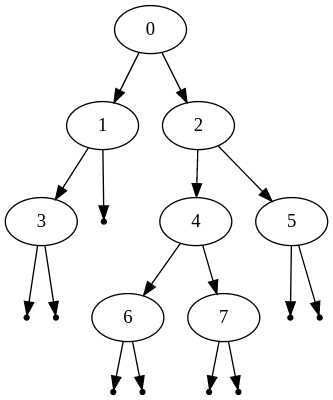
\includegraphics[scale=0.5]{images/graphviz.png}

Podemos implementar algumas funções para responder algumas perguntas sobre a nossa árvore. Por exemplo, podemos calcular o número de nós da nossa árvore.

\begin{minted}
[
frame=lines,
bgcolor=LightGray,
fontsize=\footnotesize,
linenos
]
{C++}

template <typename T> 
int btsize(NodeTree<T> * ptr){
    if(ptr == nullptr)
        return 0;
    else
        return 1 + btsize(ptr->left) + btsize(ptr->right);
}
\end{minted}


Um nó é dito ser um nó folha quando ele não possui nenhum filho (as subárvores da esquerda e direita apontam para nullptr).
A altura de um nó $v$ é o número de nós do maior caminho do nó $v$ até um nó folha descendente de $v$. A altura de uma árvore é a altura do nó raiz da árvore. 
\begin{minted}
[
frame=lines,
bgcolor=LightGray,
fontsize=\footnotesize,
linenos
]
{C++}

template <typename T> 
int btheight(NodeTree<T> * ptr){
    if(ptr == nullptr)
        return 0;
    else
        return 1 + max( btheight(ptr->left), btheight(ptr->right) );
}
\end{minted}

A profundidade de um nó $v$ é o número de nó no caminho do nó $v$ até o nó raiz. A seguinte Figura mostra uma árvore a altura e a profundidade de cada nó da árvore:

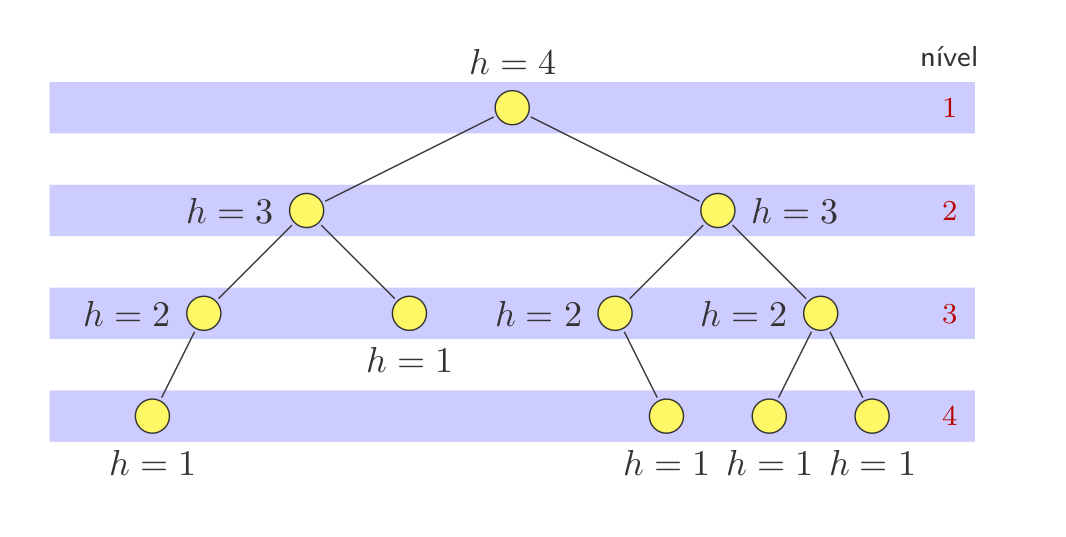
\includegraphics[scale=0.3]{images/altura.png}

\subsection{Árvore Binária Estrita}

Uma árvore binária é dita estrita quando todos os nós possuem 0 ou 2 filhos.

Seja i o número de nós internos de uma árvore binária T, n o número total de nós, l o número de folhas e $\lambda$ o número de níveis. As seguintes propriedades valem para uma árvore binária estrita:

\begin{itemize}
    \item $l = i+1$
    \item  $n = 2*i + 1$
    \item $i = (n-1)/2$
    \item $n = 2l - 1$
    \item $i = l-1$
    \item $l \leq 2\lambda - 1$
\end{itemize}





\subsection{Árvore Binária Perfeita}

Uma árvore binária é dita cheia ou perfeita se todos os nós internos tem duas folhas e todas as folhas estão no último nível.

As seguintes propriedades valem para uma árvore binária cheia:

\begin{enumerate}
    \item Se uma árvore binária cheia tem altura h então ela possui $2^{h-1}$ folhas.
    \item Se uma árvore binária cheia tem altura h então possui $2^{h} - 1$ nós.
\end{enumerate}


\fcolorbox{black}{lightblue}{
\begin{minipage}{\textwidth}
\begin{theorem}
Seja $T$ uma árvore binária cheia com altura $h$ então $T$ possui $2^{h} - 1$ nós folhas.
\end{theorem}

\begin{proof}
Considere que folhas(T) é uma função que devolve a quantidade de folhas de uma árvore de uma árvore binária T qualquer. Vamos provar por indução na altura da árvore binária cheia $T$. Se T tem altura 1, então T possui $2^{1-0}$ folhas. Por hipótese, sabemos que uma árvore binária cheia T de altura k possui $2^{k-1}$ folhas. Seja $T'$ uma árvore com altura k+1. Pela construção de uma árvore binária cheia, sabemos que as duas subárvores da esquerda e direita, respectivamente, $T_1$ e $T_2$ são cheias e possuem altura k. Por hipótese, temos que $folhas(T_1)= 2^{k-1}$ e $folhas(T_2)= 2^{k_1-1}$. Assim, 

$$folhas(T) = folhas(T_1) + folhas(T_2)$$

Dessa maneira, $folhas(T) = 2^{k} = 2^{k+1-1}$
\end{proof}


\begin{theorem}
Seja $T$ uma árvore binária cheia com altura $h$ então $T$ possui $2^{h} - 1$ nós.
\end{theorem}

\begin{proof}
Sabemos que:
\begin{itemize}
    \item Uma árvore de cheia possui $2^{0}$ nó no nível 1.
    \item Uma árvore de cheia possui $2^{2-1}$ nós no nível 2.
    \item $\ldots$
    \item Uma árvore de cheia possui $2^{h-1}$ nós no nível h.
\end{itemize}
Logo, o total de nós é $1 + 2 + \ldots 2^{h-1} = 2^h -1$
\end{proof}


\end{minipage}
}


Nós podemos usar a propriedade (2) para verificar se uma árvore binária é cheia utilizando as funções btheight e btsize.

\begin{minted}
[
frame=lines,
bgcolor=LightGray,
fontsize=\footnotesize,
linenos
]
{C++}

template <typename T>
bool is_perfect_binary(NodeTree<T> * ptr)
{
    int h = btheight(ptr);
    int n = btsize(ptr);
    return n == (1 << h) - 1;
}
\end{minted}

A seguinte árvore binária é cheia:


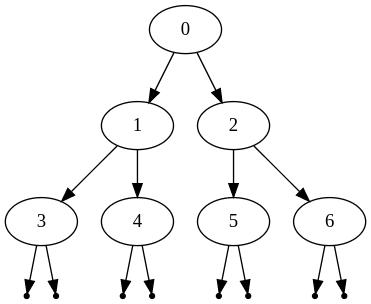
\includegraphics[scale=0.3]{images/cheia.png}

Analisando a árvore binária acima, podemos fazer uma bijeção entre a posição de um nó na árvore e a sua posição em um vetor unidimensional da seguinte maneira:

\begin{itemize}
    \item A chave da raiz será colocado na posição 0.
    \item Se a chave de um nó está na posição $i$, então a chave do filho da esquerda será colocado na posição $2i+1$ e o filho da direita será colocado na posição $2i+2$.
\end{itemize}

\subsection{Árvore Binária Completa}

Em alguns casos, a quantidade de nós não é suficiente para formar uma árvore binária cheia. Neste caso, podemos construir uma árvore binária completa. Uma árvore binária completa é uma árvore binária em que todos os níveis estão completo exceto o último nível que é preenchido da esquerda para a direita. A seguir, temos uma imagem de uma árvore completa:


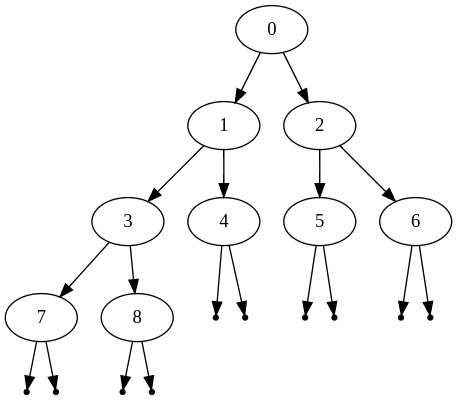
\includegraphics[scale=0.3]{images/completa.png}

Para checar se uma árvore é completa, exploraremos a relação entre a posição do nó e o seu índice em um vetor unidimensional.

\begin{minted}
[
frame=lines,
bgcolor=LightGray,
fontsize=\footnotesize,
linenos
]
{C++}

template <typename T>
bool is_complete_binary(NodeTree<T> * ptr, int index, int numnodes)
{
    if(ptr == nullptr)
        return true;
    if( index > numnodes-1)
        return false;
    else
        return  is_complete_binary(ptr->left, 2*index+1, numnodes) &&
                is_complete_binary(ptr->right, 2*index+2, numnodes);
}
\end{minted}




